\chapter{Configuring your MEGA65}
\label{cha:configuring}

\section{Preparing for First Use: Formatting SD Cards}

Depending on the model, your MEGA65 may or may not come with a pre-configured SD card.
If it doesn't, or if you wish to use a different SD card, e.g., with a
larger capacity, you must first format it for use in the MEGA65.

{\em This must be done in the MEGA65, not in a PC or other computer!}

{\em Only SDHC cards should be used. Older SD cards (typically with
  a capacity of <4GB) will definitely not work.  Newer SDXC cards with
  capacities greater than 32GB may or may not work.  We would
  appreciate hearing your experience with such cards. It also doesn't
  matter what filesystem is currently on the card, as the MEGA65
  FDISK/FORMAT utility will completely reformat the card.}

There are several reasons for this: First, in order to fit the most
features into the MEGA65's small operating system, it is a little bit
particular about the FAT32 file system it uses. Second, only the
MEGA65 FDISK/FORMAT utility can create a MEGA65 System Partition. The
MEGA65 System Partition holds non-volatile configuration settings for
your MEGA65, and also contains the freeze slots, that make it easy to
switch which programme or game you are running on your MEGA65.

Fortunately, formatting an SD card on the MEGA65 is very easy.

First, power the MEGA65 on while holding the \megakey{ALT} key down.
This should present you with the MEGA65 Utility Menu, which contains a
selection of built-in utilities, similar to the following:

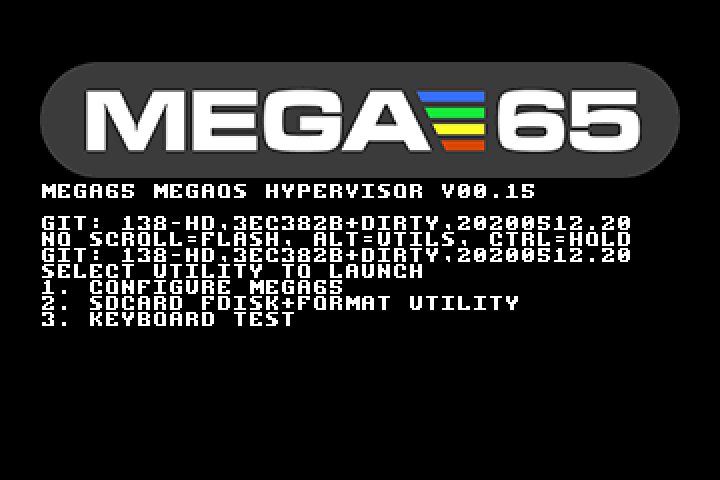
\includegraphics[width=\linewidth]{images/ss-utilmenu.png}

The exact set of utilities will
depend on the model of your MEGA65 and the version of the MEGA65
factory core which it is running. However, all versions include both
the MEGA65 FDISK/FORMAT utility, and the MEGA65 Configure utility.
Most models also include a keyboard test utility, that you can use at
any time to test that your keyboard is functioning correctly.  This is
in fact the same utility that used in the factory when testing brand
new keyboards.

Select the number that corresponds to the FDISK/FORMAT utility.  This
will typically be 2.  The FDISK utility will start, and attempt to
detect the size of any SD cards you have installed.  If you have both
an internal and external SD card installed, it will allow you to
choose which one you wish to format. The internal SD card is bus 1,
and the external card is bus 0.  But note that the MEGA65 will
always attempt to boot using an external microSD card, if one is
installed.

For safety when formatting we {\em strongly} recommend
that you remove any SD card or microSD card that you do not intend to
format, so that you can't accidentally destroy any data.  This is
because formatting an SD card in the MEGA65 cannot be undone, and you
{\em WILL} lose all data that is currently on the SD card.  If you
have any files or data on the SD card that you wish to retain, you
should first back this up somewhere.  The contents of the FAT32
partition can be easily backed up by inserting the SD card into
another computer.  The contents of the MEGA65 System Partition,
including the contents of freeze slots requires the use of specialised
software.

In generally, you should aim to backup any valuable data from your
MEGA65 on a regular basis, especially while the computer remains under
development.  While we take every care to avoid data corruption or
other mishaps, we can't guarantee that the MEGA65 is free of bugs in
this regard.

If you have only an internal SD card, you might see a
display similar to the following:

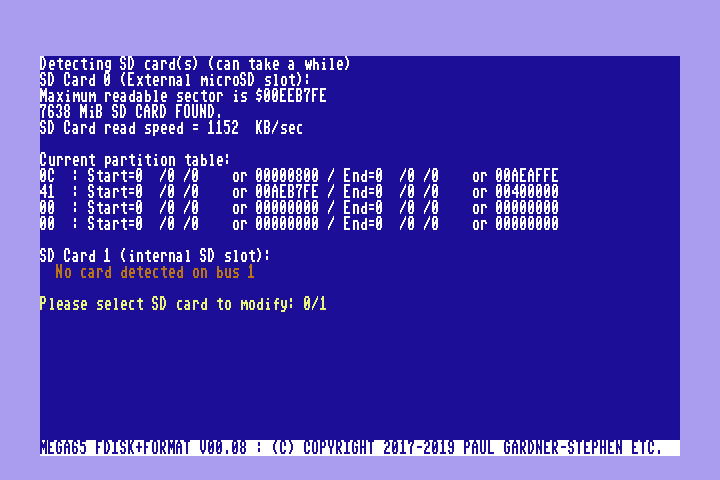
\includegraphics[width=\linewidth]{images/ss-m65fdisk-busselect.png}

Once you have selected the bus, the FDISK/FORMAT utility will ask you
to confirm that you wish to delete everything:

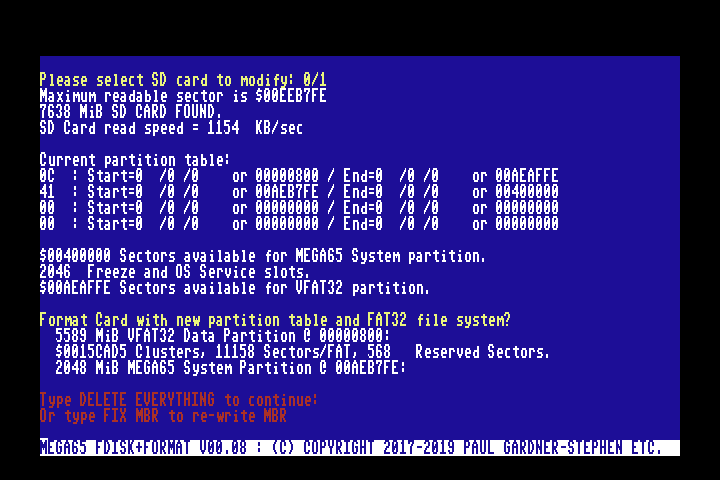
\includegraphics[width=\linewidth]{images/ss-m65fdisk-typesomething.png}

To make sure that you
know what you are doing, and don't accidentally delete everything, you
must type in ``DELETE EVERYTHING'' in capitals and press
\megakey{RETURN}.  Alternative, you can turn the MEGA65 off and on to
abort this process, without causing any damage to your data.

It is also possible to attempt to recover from a lost Master Boot
Record (``Boot Sector'') by instead typing ``FIX MBR,'' should the
need arise.

\section{Installing ROM and Other Support Files}

The MEGA65 FDISK/FORMAT utility will install a version of the
open-source OpenROM project's C64-compatible ROMs as part of the
formatting process. However, you may have other ROMs that you wish to
use on the MEGA65. The 911001 version of the C65 ROM in
particular is known to work well with the MEGA65.
You can copy as many of these as you wish onto the
SD card.  Simply make sure that they have the .ROM extension.  The ROM
you wish to use by default should be called MEGA65.ROM.  These files
should be 128KB in size, and use the same internal format as ROMs

intended for the C65.  This means that the C64-mode KERNAL should be
placed at offset \$E000, a C65-mode BASIC at \$A000, and a suitable
character set at \$D000.  

Other important files include FREEZER.M65 and AUDIOMIX.M65, which
allow you to use the MEGA65's integrated freezer.  You can download
the full set of support files for the MEGA65 from:

\url{https://github.com/mega65/mega65-files}

\section{Configuring your MEGA65}

The configuration utility for the MEGA65 fills a similar purpose to the BIOS on a
PC, and allows you to control certain default behaviours of your
MEGA65. However, rather than storing the configuration data in a
battery-backed RAM, it stores them on sector 1 of the SD card. This means
that if you switch SD cards, you will change the configuration data that you are using.

To enter the configuration utility, turn the MEGA65 on while
holding the \megakey{ALT} key.  This will show the utility menu,
similar to the following:

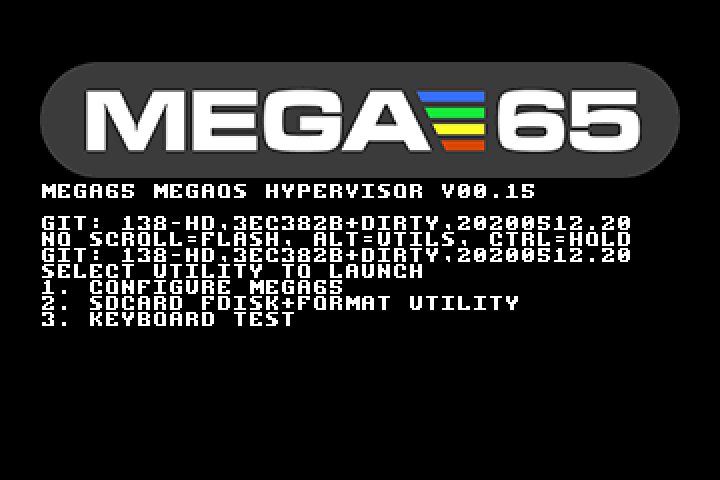
\includegraphics[width=\linewidth]{images/ss-utilmenu.png}

Now press the number corresponding to the Utility Menu.  The MEGA65
Configuration Utility will then launch, showing a display similar to
the following:

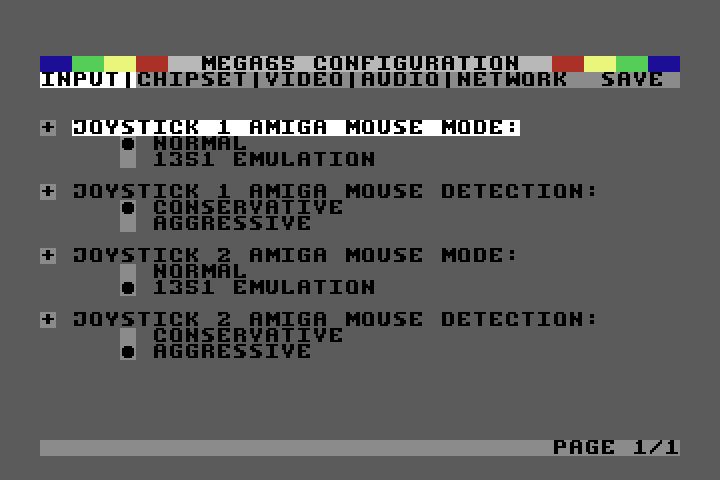
\includegraphics[width=\linewidth]{images/ss-m65config-1.png}

If your MEGA65's System Partition has become corrupt, you may be
prompted to press \megakey{F14} to correct this, i.e., hold \megakey{SHIFT} and tap
the \megakey{F13} key, with a display like the following:

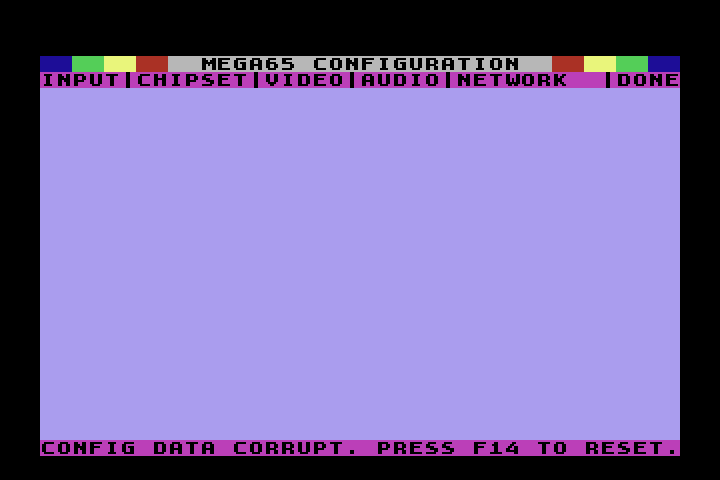
\includegraphics[width=\linewidth]{images/ss-m65config-corrupt.png}

If you do, you will
need to use \megakey{F7} to save the reset configuration, as otherwise
the reset data will not have been written back to the MEGA65 System
Partition.

Once you have dismissed that display, or if your MEGA65 System
Partition was not corrupted, you can now begin exploring and adjusting
various settings.  The programme allows the use of the keyboard, or
optionally, an Amiga(tm) or C1351 mouse to control the programme.

You can advance screens by pressing \megakey{F1}, or use \megakey{F2}
to navigate in the opposite direction through the screens. You can also
use the \megakey{$\leftarrow$} and \megakey{$\rightarrow$} keys to
navigate between the screens.

The
\megakey{$\uparrow$} and \megakey{$\downarrow$} keys can be used to
select an item.

Press \megakey{RETURN} or \megakey{SPACE} to toggle a setting, or to
allow changing a text or numeric value.  The black circle next to an
option indicates that it is the selected setting.

Finally, when you are finished, you can press \megakey{F7} to receive the
option to save the changes. This will give you four options:  

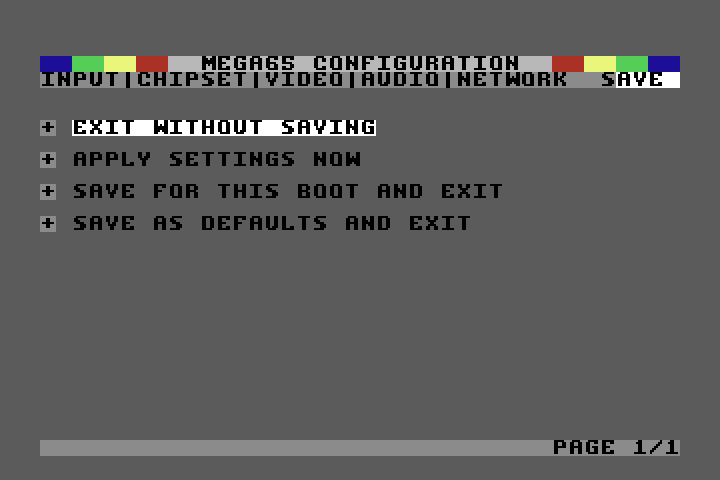
\includegraphics[width=\linewidth]{images/ss-m65config-save.png}

\begin{itemize}
  \item{\em Exit Without Saving} allows you to abandon any changes you
    have made in the MEGA65 Configure utility, without saving them.
  \item{\em Apply and Test Settings Now} makes the settings take
    immediate effect.  This can be helpful for testing compatibility
    of your TV or monitor with PAL or NTSC video modes.  If you can
    still see your display after applying such a change, you know
    that it is safe to save those settings.
  \item{\em Restore Factory Defaults} allows to you reset the
    MEGA65 configuration settings to the factory defaults. It also
    randomly selects a new MAC address for models that include an
    internal Ethernet adapter.  If you wish to commit these
    changes, you must still save them.
  \item{\em Save as Default and Exit} commits any changes you
    have made to the SD card storage, so that they will be used
    by your MEGA65 whenever you turn it on.
\end{itemize}

\subsection{Input Devices}

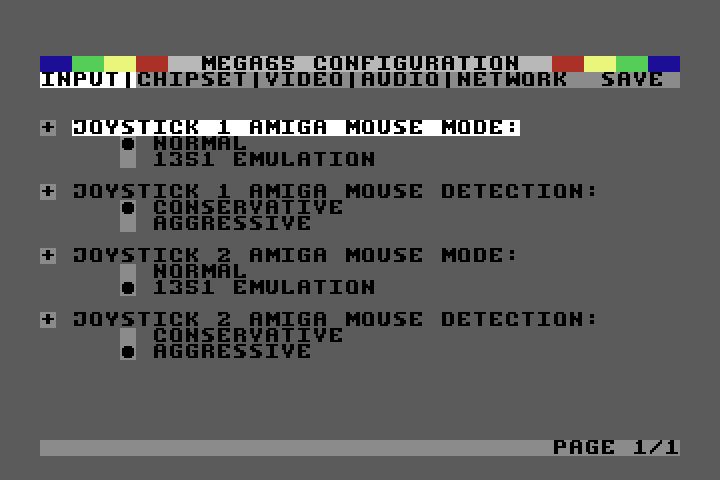
\includegraphics[width=\linewidth]{images/ss-m65config-1.png}

\begin{itemize}
  \item{\em Joystick 1 Amiga Mouse Mode} allows either {\bf normal} operation,
    where software will see it as an Amiga mouse, or {\bf 1351
      emulation} mode, where the MEGA65 translates the Amiga mouse's
    movements into 1351 compatible signals. This allows you to use an
    Amiga mouse with existing C64/C65 software that expect a 1351
    mouse.
  \item{\em Joystick 1 Amiga Mouse Detection} can be set to conservative
    or aggressive.  If you use an Amiga mouse, and it fails to move
    smoothly in all directions, you may wish to set it to {\bf
      aggressive}. Conversely, if you regularly use joysticks in the
    port, and have difficulties with the joystick input
    mis-behaving, you may wish to select the {\bf conservative}
    option.
  \item{\em Joystick 2 Amiga Mouse Mode} is the same as the first
    option, but for the second joystick port. This allows you to
    have different policies for each port.
  \item{\em Joystick 2 Amiga Mouse Detection} similarly provides the
    ability to separately control the Amiga mouse detection
    algorithm for the second joystick port.
\end{itemize}


\subsection{Chipset}

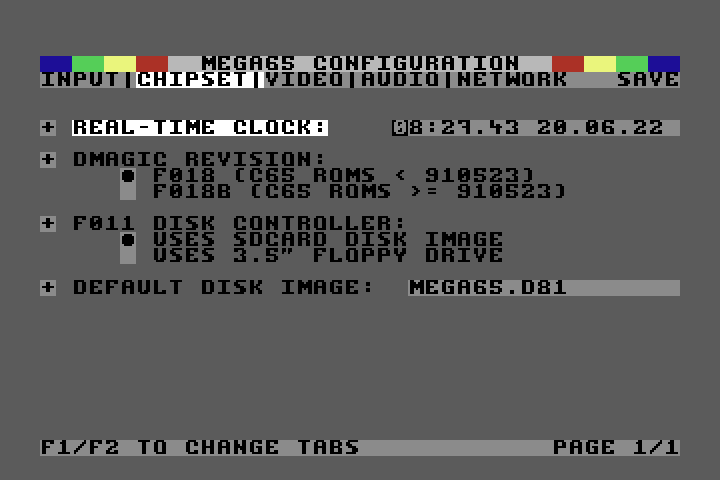
\includegraphics[width=\linewidth]{images/ss-m65config-2.png}

\begin{itemize}
  \item{\em DMAgic Revision} allows selecting the default mode of
    operation for the C65 DMAgic DMA controller.  This option is only
    required for ROMs that the MEGA65's HYPPO Hypervisor does not
    detect.  If you see screen corruption in BASIC, you may wish to
    try toggling this option.
  \item{\em F011 Disk Controller}
    This option allows you to select whether the internal 3.5'' floppy
    drive functions using real diskettes, or whether it simply makes
    noises to add atmosphere when using D81 disk images from the SD
    card.  This merely sets the default option, and you can change
    this setting, or select a different disk image for use as either
    or both of the C65 3.5'' DOS based drives.
  \item{\em Default Disk Image} allows you to choose the D81 disk image
    that will be used with the internal drive, if the F011 Disk
    Controller option above is set to use an SD card disk image.    
\end{itemize}

\subsection{Video}

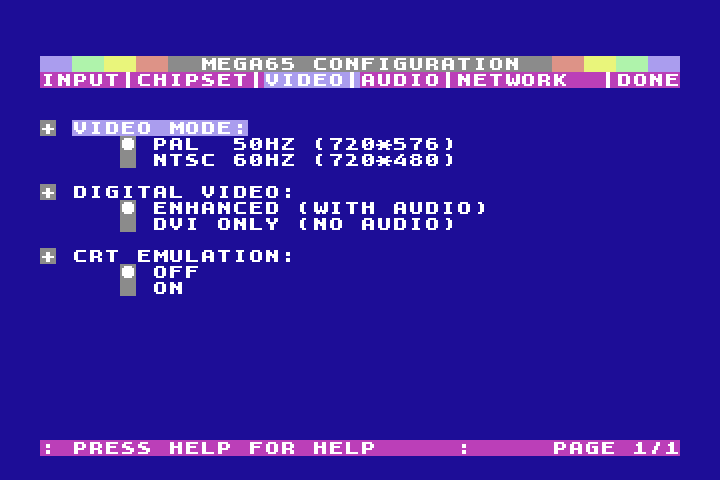
\includegraphics[width=\linewidth]{images/ss-m65config-3.png}

\begin{itemize}
  \item{\em Video Mode} selects whether the MEGA65 starts in PAL or NTSC.
    The MEGA65 supports true 480p NTSC and 576p PAL double-scan modes,
    with exact 60Hz / 50Hz frame-rates.  This setting merely sets the
    default value, and the system can be switched between PAL and NTSC
    via the Freeze Menu, or under software control by MEGA65-enabled
    programmes.
\end{itemize}

\subsection{Audio}

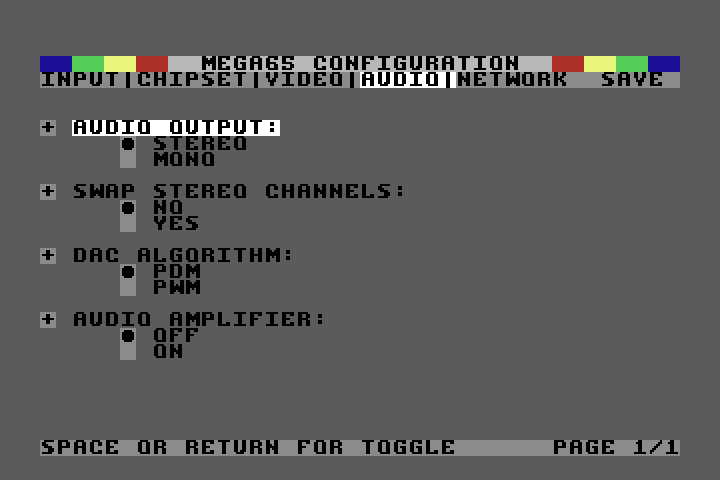
\includegraphics[width=\linewidth]{images/ss-m65config-4.png}

\begin{itemize}
  \item{\em Audio Output} selects whether the SIDs and digital audio
    channels are combined to provide a mono-aural signal, or whether
    the left and right tagged audio sources are separated to provide a
    stereo signal. Again, this setting can be varied from in the Audio
    Mixer of the Freeze Menu, or under the control of MEGA65-enabled
    software.
  \item{\em Swap Stereo Channels} allows switching the left and right
    sides of the stereo audio output. This is primarily useful for
    software that expects left and right SIDs to be at swapped
    addresses compared with the MEGA65.
  \item{\em DAC Algorithm} allows selecting between two different
    digital to analog conversion algorithms.  Both are very good,
    but you may have a preference for one or the other.
  \item{\em Audio Amplifier} allows enabling or disabling the audio
    amplifier that is contained in some models of the MEGA65 for
    certain audio outputs, e.g., internal speaker or loud speaker.
\end{itemize}

\subsection{Network}

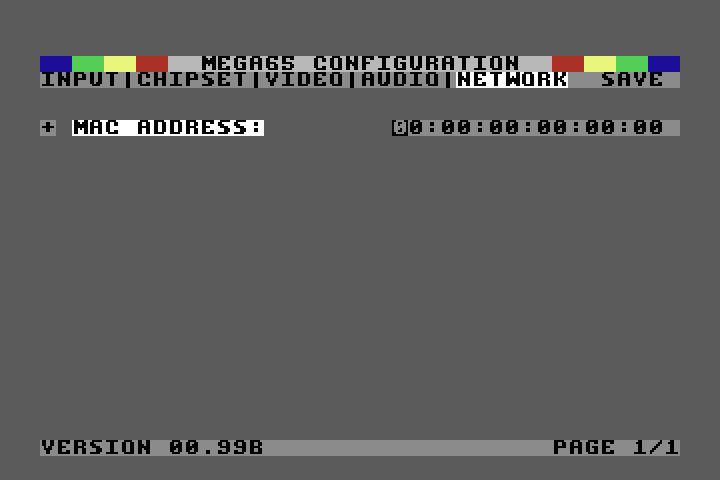
\includegraphics[width=\linewidth]{images/ss-m65config-5.png}

\begin{itemize}
  \item{\em MAC Address} allows you to set the default MAC address of your
    MEGA65.  This can be changed at run-time by MEGA65-enabled
    software
\end{itemize}
